\section{Transistoren}

\subsection{Bipolar-Transistor (BJT)}
Die BJT bestehen aus 2 Dioden, durch das Anlegen einer Spannung $V_{BE} \approx 0.7V$ wird die untere Diode leitend. 
Die Elektronen gelangen in die p-Schicht und werden dort vom Pluspol der Spannung $V_{BE}$ angezogen (ca. $1\%$ Elektronen). Da diese nur sehr klein ist, wandern die Elektronen 
in die obere Schicht und werden dort vom Pluspol der Spannung $V_{CE}$ angezogen (ca. $99\%$ Elektronen). Es fliesst der Strom $I_C = \beta \cdot I_{BE}$. Weil $\beta$ meist sehr gross ist, 
kann der Basisstrom meistens vernachlässigt werden.

\begin{center}
	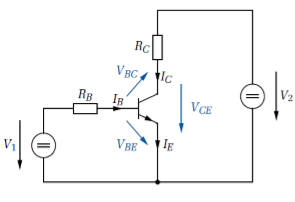
\includegraphics[width=0.5\columnwidth]{Images/bipolar}
\end{center}

\noindent Der BJT-Transistor ist folgendermassen beschrieben:
\begin{minipage}{0.20\textwidth}
	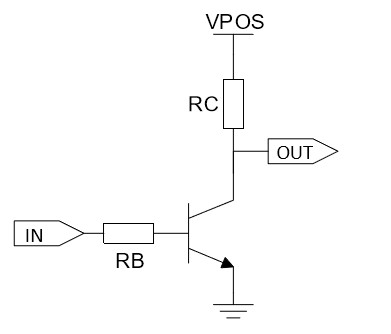
\includegraphics[width=\linewidth,keepaspectratio=true]{./Images/bjt}
\end{minipage}%%% to prevent a space
\begin{minipage}{0.30\textwidth}
	\begin{align*}
		A &= \frac{\partial V_{out}}{\partial V_{in}} = \frac{-R_C \cdot I_C}{n\cdot V_T}  \\
		V_{out} &= V_{pos} - R_C\cdot\beta\cdot I_s\cdot e^{\frac{V_{in}}{n\cdot V_T}}
	\end{align*}
\end{minipage}

\noindent Der Kleinsignalwiderstand $R_{BE}$ kann ist folgend definiert Siehe auch Kapitel \ref{dioden}: \[R_{BE} = \frac{m\cdot V_T}{I_{B0}}\]

\subsubsection{Early-Spannung}
Die Early-Spannung kann durch die Geradengleichung berechnet werden. Es werden zwei punkte im Lineren Bereich extrapoliert und mit der x-Achse geschnitten.
\[
R_{CE} \approxeq \frac{V_A}{I_C}
\]
\begin{center}
	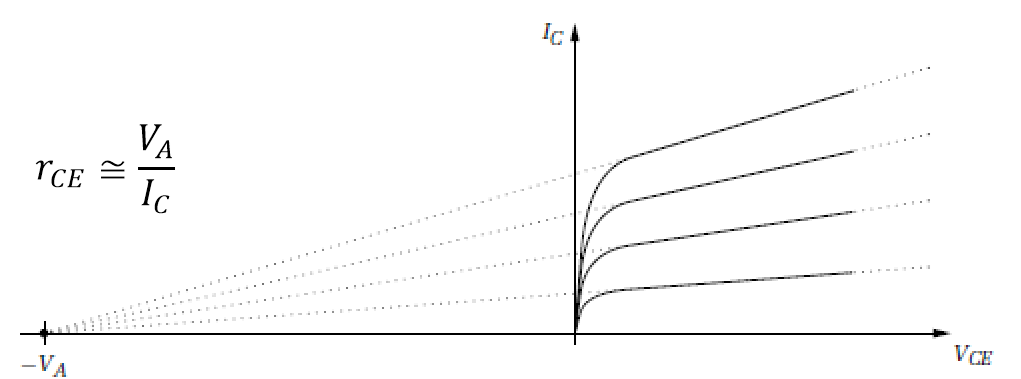
\includegraphics[width=0.7\columnwidth]{Images/early-spannung}
\end{center}


\subsubsection{Thermischer Widerstand}
Mit dem Thermische Widerstand $R_{th}$ kann die Temperaturänderen $\Delta T = R_{th} \cdot P$ berechnet werden. Die Maximale Leistung mit Umgebungstemperatur $R_{th}$: \[P_{max} = \frac{T_{max} - T_U}{R_{th}}\]

\subsubsection{Ausgangsstufen}
Mit BJT-Transistoren können Verstärker gebaut werde wobei die Effizient $\eta = \frac{P_{AC}}{P_B + P_{DC}} \approx \frac{P_{AC}}{P_{DC}}$ ist.
\begin{center}
	\includegraphics[width=0.5\columnwidth]{Images/verstärker-typen}
\end{center}

\textbf{Class-A Verstärker}\\
Einfach, kleinste Verzezzunr, aber viel DC-Strom, was zu einem schlechten Wirkungsgrad führt $\eta \approx 25\%$ \\
\begin{minipage}{0.20\textwidth}
	\includegraphics[width=\linewidth,keepaspectratio=true]{Images/verstärker-typen1}
\end{minipage}%%% to prevent a space
\begin{minipage}{0.30\textwidth}
	\begin{align*}
		P_{AC_{max}} &= \frac{V_{max}}{\sqrt{2}}\cdot \frac{\hat{I}_{max}}{\sqrt{2}} \\
		P_{DC} &= V_{POS} \cdot I_L \xRightarrow{I_L = \frac{V_{POS}}{2\cdot R_L}} \frac{V_{POS}^2}{2\cdot R_L}
	\end{align*}
\end{minipage}

\textbf{Class-B Verstärker}\\
Ist Effizient, verzerrt Signal um 0V. Wirkungsgrad $\eta \approx 78.5\%$\\
\begin{minipage}{0.20\textwidth}
	\includegraphics[width=\linewidth,keepaspectratio=true]{Images/verstärker-typen2}
\end{minipage}%%% to prevent a space
\begin{minipage}{0.30\textwidth}
	\begin{align*}
		P_{AC_{max}} &= \frac{V_{max}^2}{2 \cdot R_L} \\
		P_{DC} &= \frac{2}{\pi}\frac{V_{POS}\cdot V_{max}}{R_L}
	\end{align*}
\end{minipage}

\textbf{Class-AB Verstärker}\\
Guter Kompromiss von A und B Verstärker\\
\begin{minipage}{0.20\textwidth}
	\includegraphics[width=\linewidth,keepaspectratio=true]{Images/verstärker-typen3}
\end{minipage}%%% to prevent a space
\begin{minipage}{0.30\textwidth}
\end{minipage}


\subsubsection{Ersatzschaltbild}
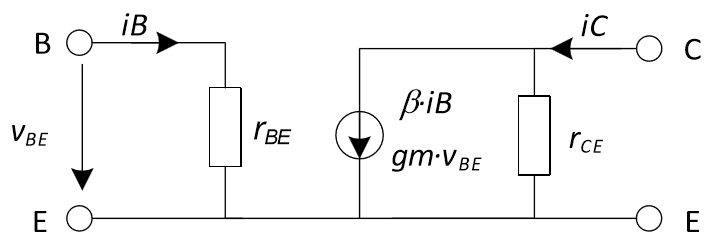
\includegraphics[width=\linewidth,keepaspectratio=true]{Images/bjt_esb}

\subsection{Schaltungen}
\textbf{Widlar-Stromspiegel}\\
\begin{minipage}{0.20\textwidth}
	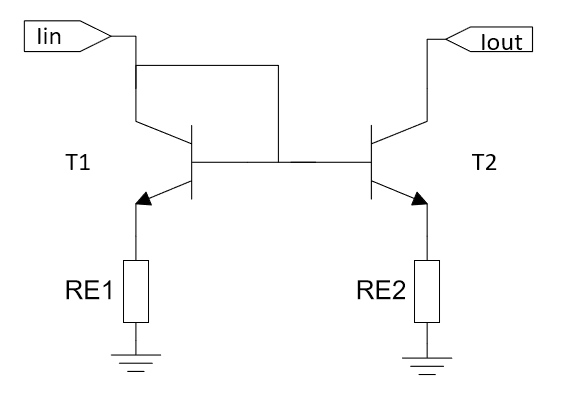
\includegraphics[width=\linewidth,keepaspectratio=true]{Images/widlar-stromspiegel}
\end{minipage}%%% to prevent a space
\begin{minipage}{0.30\textwidth}
	\begin{align*}
		V_{E1} &= R_{E1}\cdot I_{in} \approx V_{E2} \\
		V_{B1} &= V_{B2} = V_{E1}+V_{BE0} \\
		&\xRightarrow[]{} I_{E2} = \frac{V_{E2}}{R_{E2}} \\
		I_{out} &= I_{in} \cdot \frac{R_{E1}}{R_{E2}}
	\end{align*}
\end{minipage}\\
\textbf{Differenzverstärker}\\
\begin{minipage}{0.20\textwidth}
	\includegraphics[width=\linewidth,keepaspectratio=true]{Images/diffverstärker}
\end{minipage}%%% to prevent a space
\begin{minipage}{0.30\textwidth}
	\begin{align*}
		\frac{I_{C1}}{I_{C2}} = e^{\frac{V_D}{n\cdot V_T}}
	\end{align*}
\end{minipage}
\begin{minipage}{0.20\textwidth}
	\includegraphics[width=\linewidth,keepaspectratio=true]{Images/diffverstärker1}
\end{minipage}%%% to prevent a space
\begin{minipage}{0.30\textwidth}
	\begin{align*}
		I_{C1} &= I_{BIAS} \cdot e^{\frac{V_D}{n\cdot V_T}} \cdot \frac{1}{e^{\frac{V_D}{n\cdot V_T}} + 1} \\
		I_{C2} &= I_{BIAS} \cdot \frac{1}{e^{\frac{V_D}{n\cdot V_T}} + 1} \\
	\end{align*}
\end{minipage}
\begin{minipage}{0.20\textwidth}
	\includegraphics[width=\linewidth,keepaspectratio=true]{Images/diffverstärker2}
\end{minipage}%%% to prevent a space
\begin{minipage}{0.30\textwidth}
	\begin{align*}
		S_{x} &= \frac{I_{Cx}}{m\cdot V_T} \qquad V_{BE} = \frac{\Delta V_{in}}{2} \\
		V_{out} &= \frac{\Delta V_{in}}{2} S_{T1}R_{C1} + \frac{\Delta V_{in}}{2} S_{T2}R_{C2}
	\end{align*}
\end{minipage}




\subsection{JFET}
Bei einem Feldeffekttransistor wird der Stromfluss durch den leitenden Kanal mittels eines elektrischen Feldes gesteuert. Die p-leitende Schicht ist als Gate-Anschluss aus dem Bauteil geführt. Wenn an Drain und Source eine Spannung angelegt wird fliesst ein Strom von Source zu Drain. Die n-leitende Schicht hat gegenüber den p-leitenden Schichten eine positive Spannung. Um die p-leitenden Zonen entsteht eine Sperrschicht. Die Breite der Sperrschichten nimmt mit der an Source und Drain anliegenden Spannungshöhe im n-Kanal zu. Innerhalb der Sperrschichten befinden sich keine frei beweglichen Ladungsträger. Die Elektronen im n-Kanal müssen den Weg zwischen den Sperrschichten nehmen. Die \underline{doppelte Verstärkung} benötigt den 4-fachen Strom.

Die Sperrschicht steuert einen Widerstand im linearen Bereich. Dabei sind $I_{DSS}$ und Pinch-Off-Spannung $V_P$ Technologieparameter.
\[
I_D = \frac{2I_{DSS}}{V_p^2}\left(V_{GS} - V_P - \frac{V_{DS}}{2}\right)V_{DS}
\]
Für den Stromquellenbereich muss folgende Formel verwendet werden:
\[
I_D = \frac{I_{DSS}}{V_P^2}\left(G_{GS} - V_P\right)^2
\]

\subsection{MOSFET}
Der Transistor befindet sich im Sperr-Zustand (deshalb selbstsperrend), wenn keine positive Spannung zwischen Gate- und Source-Anschluss anliegt. Wird zwischen Gate und Source eine positive Spannung $V_{GS}$ angelegt, dann entsteht im Substrat ein elektrisches Feld. Die Elektronen werden vom Gate-Anschluss aus dem p-leitende Substrat (viele Löcher, sehr wenige Elektronen) angezogen. Sie wandern bis zur Isolierschicht. Die Löcher wandern in entgegengesetzter Richtung. Die Zone zwischen den n-leitenden Inseln enthält überwiegend Elektronen als freie Ladungsträger. Zwischen Source- und Drain-Anschluss befindet sich nun ein n-leitender Kanal. Die Leitfähigkeit dieses Kanals lässt sich durch die Gatespannung $V_{GS}$ steuern.
Mosfet arbeitet als spannungsgesteuerte Widerstand mit Breite $W$ und Länge $L$.
\[
I_D = \beta \cdot \left(V_{GS} - V_{TH} \frac{V_{DS}}{2}\right)\cdot V_{DS} \qquad \beta = \frac{W}{L}C_{ox}\mu_n
\]
Andernfalls ist Mosfet im Sättigungsbereich als spannungsgesteuerte Stromquelle
\[
I_D = \frac{\beta}{2}\left(V_{GS} - V_{TH}\right)^2
\]